\documentclass[11pt,letterpaper]{article}

\usepackage[margin=1in]{geometry}
\usepackage[T1]{fontenc}
\usepackage[utf8]{inputenc}
\usepackage{lmodern}
\usepackage{microtype}
\usepackage{amsmath,amssymb,amsthm}
\usepackage{booktabs,longtable,array}
\usepackage{xcolor}
\usepackage{graphicx}
\usepackage{listings}
\usepackage{enumitem}
\usepackage{hyperref}
\usepackage{titlesec}
\usepackage{fancyhdr}

\hypersetup{
  colorlinks=true,
  linkcolor=black,
  citecolor=black,
  urlcolor=blue,
  pdfauthor={Generative AI (Claude Opus 4.8), revised with literature grounding},
  pdftitle={What Was Conceptually New in SHACL? A Calibrated Re-examination against RacerPro nRQL}
}

\pagestyle{fancy}
\fancyhf{}
\lhead{SHACL vs.\ nRQL (revised)}
\rhead{\thepage}
\setlength{\headheight}{14pt}

\titleformat{\section}{\large\bfseries}{\thesection}{0.7em}{}
\titleformat{\subsection}{\normalsize\bfseries}{\thesubsection}{0.7em}{}
\titleformat{\subsubsection}{\normalsize\itshape}{\thesubsubsection}{0.7em}{}

\theoremstyle{definition}
\newtheorem{lemma}{Lemma}
\newtheorem{proposition}{Proposition}
\newtheorem{remark}{Remark}

\lstdefinelanguage{nrql}{
  morekeywords={retrieve,and,union,neg,NEG,not,NOT,project-to,project,pi,substitute,firerule,defquery,instance,related,constrained,constraints,in-tbox,in-abox,in-mirror-data-box,enable-data-substrate-mirroring,enable-smart-abox-mirroring,has-known-successor,same-as,NIL,TOP,BOTTOM},
  sensitive=false,
  morecomment=[l]{;},
  morestring=[b]"
}
\lstdefinelanguage{turtle}{
  morekeywords={a,prefix,BASE,PREFIX,true,false},
  sensitive=true,
  morecomment=[l]{\#},
  morestring=[b]"
}
\lstset{
  basicstyle=\small\ttfamily,
  columns=fullflexible,
  keepspaces=true,
  showstringspaces=false,
  breaklines=true,
  frame=single,
  framerule=0.2pt,
  xleftmargin=0.5em,
  xrightmargin=0.5em
}

\newcommand{\nrql}{nRQL}
\newcommand{\racer}{RacerPro}
\newcommand{\shacl}{SHACL}
\newcommand{\naf}{negation as failure}
\newcommand{\abox}{ABox}
\newcommand{\tbox}{TBox}
\newcommand{\rdf}{RDF}
\newcommand{\owl}{OWL}

\begin{document}

\begin{titlepage}
  \centering
  \vspace*{1.1in}
  {\LARGE \bfseries What Was Conceptually New in SHACL?\par}
  \vspace{0.25in}
  {\Large \bfseries A Calibrated Re-examination against RacerPro \nrql{},\par}
  {\Large \bfseries Negation as Failure, and the Data Substrate\par}
  \vspace{0.5in}
  {\large Revised edition, with independent literature grounding\par}
  \vspace{0.9in}
  {\large Prepared from the RacerPro manuals, the \shacl{} specifications,\par}
  {\large and primary sources in the description-logic and \rdf{}-validation literature\par}
  \vspace{0.45in}
  {\large Drafted by a generative AI system (Claude Opus 4.8)\par}
  {\normalsize and substantiated against cited publications; see the authorship declaration.\par}
  \vfill
  {\large \today\par}
\end{titlepage}

\pagenumbering{roman}
\begin{abstract}
This report re-examines a specific historical-semantic question: what did \shacl{} make expressible as a constraint language that was not already expressible, in principle, in \racer{} via \nrql{}, \naf{} (NAF), projection, rules, concrete-domain/datatype predicates, and the substrate / \owl{}\,data-mirroring layer? It revises an earlier draft in four ways. First, it grounds the priority discussion in the description-logic literature rather than in the vendor manual alone: the idea of querying ``what is known'' through an epistemic / minimal-knowledge operator was formalized by Donini et al.\ in 1998 \cite{epistemic}, and the ``effective first-order query'' agenda was crystallized by EQL-Lite in 2007 \cite{eqllite}; \nrql{} (2004--2005) \cite{adl04,nrql05} sits between them as, defensibly, the first \emph{practical, high-performance} engine to offer \naf{} plus projection over an \owl{} knowledge base. Contemporary \rdf{} query languages such as RQL (2002) \cite{rql} and RDQL (January 2004) \cite{rdql} did not offer negated projected subqueries (RDQL admitted only ``safe'' negation with no variables in the negated clause). This supports a \emph{prior-art} and \emph{conceptual-anticipation} claim, but not a claim of \emph{documented influence} on SPARQL~1.1, \shacl{}, or property-graph languages, and not a claim of global ``firstness.''

Second, it replaces the earlier ``informal expressivity theorem''---which assumed away exactly the hard cases---with an explicit \emph{reduction lemma} whose stated assumptions mark the true boundary of the comparison. Third, it sharpens what is genuinely new in \shacl{} to two items with rigorous backing rather than one: (i)~a \emph{recursive} shape-conformance relation, whose semantics is a nontrivial object (partial / stable / well-founded assignments) and whose associated decision problems can be NP-hard or undecidable \cite{recshacl,stableshacl,satcont}; and (ii)~\emph{unbounded regular property paths}, which are provably beyond the nonrecursive \naf{}-plus-projection fragment because transitive closure is not first-order definable \cite{ahoullman,libkin}. \rdf{}-term-native components (node kind, language tags, lexical form) and \shacl{}'s validation-report vocabulary are conditional or organizational differences. Fourth, it adds a section on three \emph{semantic traps} in the naive translation---epistemic-mode mismatch, cardinality counting without a unique-name assumption, and the active-domain-versus-anonymous-witness gap---that the earlier draft underweighted.

The net conclusion is unchanged in spirit but more precise: the large majority of recurring \emph{OWL-centric, finite, closed-world} integrity checks that \shacl{} is used for were already within reach of \nrql{} plus the mirror substrate by 2005, and \nrql{} deserves explicit recognition as prior art for negated projected subqueries in a practical \owl{} query engine. In place of the earlier draft's bare ``$80\%$'' we report an empirical \emph{band} from coding the W3C \shacl{} test suite (\S\ref{sec:empirical}): \textbf{73--84\%} of \shacl{} Core constraint features have a direct \nrql{} counterpart ($\approx\!92\%$ once the substrate mirror is granted), while the \emph{provably} native residual is only $\approx\!5\%$ (unbounded/recursive paths, matching Proposition~\ref{prop:paths}), rising to a best estimate of $\approx\!8\%$ once \texttt{sh:pattern} regular expressions are counted---which RacerPro cannot express \emph{declaratively}. Crucially, \nrql{}'s lambda/\texttt{:reject} hatch is \racer{}'s deliberately \emph{termination-safe} ``MiniLisp''---not Turing-complete (recursion is aborted at runtime; no regex engine), as we confirmed live on \racer{}~2.0---so, unlike \shacl{}'s own (Turing-complete) SPARQL/JS hatches, it does \emph{not} close the residual: unbounded paths and full-regex patterns survive it. That termination guarantee is the principled choice for a decidable DL query engine. We also \emph{correct} the earlier draft's property-graph stance (\S\ref{sec:declined}): the data substrate is a genuine, reasoning-coupled property graph with first-class, queryable edge property maps---real prior art for property-graph modeling fused with DL reasoning---though the attributed-graph model class predates it (1984--1994) and we find no documented influence on later property-graph languages. The residual novelty of \shacl{} is concentrated, precisely, in recursive shape conformance, native regular-path validation, \rdf{}-term primitives, and the standardized conformance/report model.
\end{abstract}

\section*{Generative AI authorship and independence declaration}\label{sec:ai-declaration}
\addcontentsline{toc}{section}{Generative AI authorship and independence declaration}
This report was drafted by a generative AI system (Claude Opus 4.8). The human user supplied the research question, the RacerPro manuals, and a request to substantiate or disprove the priority claims using external sources. Those inputs were treated as material and hypotheses to be tested, not conclusions to be adopted. Where the user's earlier draft proposed a figure (``80\%''), a property-graph priority claim, or an ``informal theorem,'' this revision either qualifies, rescopes, or withdraws the claim and says so explicitly. Bibliographic claims about dates and contents were checked against the cited publications; the description-logic and \rdf{}-validation references below were located through literature search rather than supplied by the user. The report credits \racer{}/\nrql{} as strong prior art where the manuals and the dated publications support it, and it does not assert documented causal influence on later standards absent a citation trail.

\tableofcontents
\newpage
\pagenumbering{arabic}

\section{Question, scope, and what changed}\label{sec:scope}

The question is conceptual, not sociological. It is \emph{not} whether \shacl{} became a W3C standard, attracted more implementations, or integrated better with generic \rdf{} tooling; those are real and important facts, and they are out of scope here. The question is:

\begin{quote}
What did \shacl{} make expressible as a constraint language that was not already expressible, in principle, in \racer{} by \nrql{} plus the substrate representation layer, the mirror data substrate, and hybrid \nrql{} queries?
\end{quote}

This revision differs from the earlier draft in four substantive ways, each justified in the body:
\begin{enumerate}[leftmargin=2em]
  \item \textbf{Priority is grounded in the literature, not the manual alone} (\S\ref{sec:priority}). The manual's self-description (``the only practically available \owl{} query language of its time'' for autoepistemic queries \cite[p.~82]{racerug}) is a vendor claim. We keep it, but we anchor the substantive priority claim in dated, independent publications and name the contemporaries it is implicitly measured against.
  \item \textbf{The ``informal theorem'' becomes an explicit reduction} (\S\ref{sec:reduction}) whose assumptions are the point.
  \item \textbf{Two genuine novelties, with proofs/citations, not one} (\S\ref{sec:new}): recursive shape conformance and unbounded regular paths.
  \item \textbf{A new section on translation traps} (\S\ref{sec:traps}), \textbf{withdrawal of the ``80\%'' figure} (\S\ref{sec:headline}), and a \textbf{corrected, evidence-based property-graph assessment} (\S\ref{sec:declined}).
\end{enumerate}

Throughout, ``possible with \nrql{}'' is read generously, matching the system the manuals describe: \abox{} queries with classical negation, \naf{}, projection, union, and conjunction; DL-aware atoms evaluated by entailment; rules with query-body antecedents and generalized \abox{} consequents; concrete-domain/datatype predicates; group-by and aggregation; complex \tbox{} queries; hybrid \abox{}-plus-substrate queries; and the mirror data substrate for \owl{} documents, annotations, and told datatype/annotation values \cite[pp.~4,\,81--84,\,113--143]{racerug}. On the \shacl{} side we distinguish \shacl{} Core, \shacl{}-SPARQL, and \shacl{} Advanced Features \cite{shacl,shaclaf}.

\section{Background, compressed}\label{sec:background}

\subsection{nRQL's epistemic profile}
\nrql{} query bodies are built compositionally with \texttt{and}, \texttt{union}, \texttt{neg}, and \texttt{project-to} \cite[pp.~81--82]{racerug}. A \emph{positive} atom binds a variable only to individuals for which the atom, after substitution, is \emph{logically entailed} by the \racer{} knowledge base \cite[p.~82]{racerug}; positive atoms are therefore open-world and DL-aware. The \texttt{neg} constructor is \naf{}: it succeeds when the enclosed body has no answer over the active domain of \emph{known} individuals (or substrate nodes) \cite[pp.~113--117]{racerug}. Crucially, \texttt{project-to} may appear \emph{inside} a body, so \naf{} can be applied to a projected subquery---an anti-semi-join / \texttt{NOT EXISTS} pattern. This hybrid---open-world entailment for positive atoms, closed-world failure for selected subexpressions---is exactly the ``autoepistemic'' profile the manual advertises \cite[p.~82]{racerug}, and it is the technical heart of the comparison.

\subsection{The substrate and the mirror}
A \emph{data substrate} is a node- and edge-labeled directed graph whose labels are Lisp symbols, strings, numbers, and characters \cite[p.~133]{racerug}; a substrate may be associated with an \abox{} so that \nrql{} becomes a \emph{hybrid} query language addressing both \cite[pp.~133--137]{racerug}. The \emph{mirror data substrate} automatically materializes substrate objects for \abox{} individuals and, for an \owl{} KB, for \owl{} elements---adding markers such as \texttt{:owl-annotation}, \texttt{:owl-annotation-relationship}, \texttt{:owl-annotation-value}, \texttt{:owl-datatype-value}, and \texttt{:owl-datatype-role}---so that annotations and told datatype/annotation fillers become \emph{queryable data} \cite[pp.~137--143]{racerug}. This is the single most under-appreciated fact for a fair comparison: it refutes the common claim that \nrql{} was ``only'' an \abox{} query language unable to reach ontology metadata.

\subsection{SHACL, compressed}
\shacl{} Core defines \emph{shapes} (node and property shapes) with constraint components (\texttt{sh:minCount}, \texttt{sh:maxCount}, \texttt{sh:class}, \texttt{sh:datatype}, \texttt{sh:nodeKind}, \texttt{sh:pattern}, \texttt{sh:languageIn}, \texttt{sh:closed}, logical combinators, qualified value shapes, property paths). Its primary semantic object is a \emph{conformance} relation between a data graph and a shapes graph, with structured \emph{validation results} for non-conformances \cite{shacl}. \shacl{}-SPARQL allows constraints written as SPARQL queries; \shacl{} Advanced Features adds rules \cite{shaclaf}. \shacl{}'s visible design lineage runs through SPIN \cite{spin}, OSLC Resource Shapes, and Shape Expressions (ShEx) \cite{shex}, not through DL query languages.

\section{Historical priority, done carefully}\label{sec:priority}

\subsection{Three claims, kept separate}
Following standard practice we separate:
\begin{enumerate}[leftmargin=2em]
  \item \textbf{Prior art:} \nrql{} had a feature before a later language standardized or popularized a similar one.
  \item \textbf{Conceptual convergence:} two communities independently built similar mechanisms because they faced the same finite-graph constraint problem.
  \item \textbf{Direct influence:} designers of the later language knew of, cited, or built on \nrql{}.
\end{enumerate}
Only the first is strongly supported here; the second is plausible; the third we do not assert.

\subsection{What the idea owes to earlier DL work}
Intellectual honesty requires noting that \nrql{} did not invent the \emph{idea} of asking a DL knowledge base ``what is known.'' Donini, Lenzerini, Nardi, Nutt and Schaerf formalized an \emph{epistemic operator} $\mathbf{K}$ for description logics in 1998, explicitly to capture queries, procedural rules, and closed-world reasoning over an open-world KB \cite{epistemic}; the minimal-knowledge / \naf{} semantics was further developed in the MKNF line \cite{mknf}. \nrql{}'s contribution is therefore not the concept of autoepistemic querying but its \emph{practical realization}: a high-performance engine in which \naf{}, projection, aggregation, rules, and concrete-domain predicates are available together over real \owl{} data, benchmarked on LUBM \cite{adl04,nrql05}. Read this way, the priority claim becomes both more modest and more defensible.

\subsection{What the dated record supports}
The \nrql{} idiom that matters is \texttt{NEG} over a projected (or named) query body:
\begin{lstlisting}[language=nrql,caption={nRQL negated projected query body: an anti-existential subquery.}]
(retrieve (?x)
  (neg (project-to (?x)
         (and (?x c) (?x ?y r) (?y d)))))
\end{lstlisting}
\begin{lstlisting}[language=nrql,caption={NAF applied to a defined query body.}]
(defquery mother-of (?x ?y)
  (and (?x woman) (?x ?y has-child)))
(retrieve (?a ?b)
  (neg (substitute (mother-of ?a ?b))))
\end{lstlisting}
These appear in the user's guide \cite[pp.~119--122]{racerug} and the mechanism is described in the dated 2004--2005 publications \cite{adl04,nrql05}. The relevant comparison dates are: RQL, 2002 \cite{rql}; RDQL, W3C Member Submission of 9~January 2004 \cite{rdql}; \nrql{}, ADL'04 (September 2004) and DL~2005 \cite{adl04,nrql05}; EQL-Lite, IJCAI~2007 \cite{eqllite}; SPARQL~1.0, W3C Recommendation 2008 \cite{sparql10}; SPARQL~1.1 (with \texttt{FILTER NOT EXISTS}, \texttt{MINUS}, subqueries), 2013 \cite{sparql}; \shacl{}, 2017 \cite{shacl}.

Against the contemporaries this yields a concrete, checkable contrast rather than a bare assertion of firstness:
\begin{itemize}[leftmargin=2em]
  \item \textbf{RQL (2002)} is a declarative, schema-aware \rdf{} query language built around class/property/value navigation; it does not provide a general \naf{}-over-projection (negated subquery) construct for ``no known $r$-successor satisfying $\varphi$.''
  \item \textbf{RDQL (Jan 2004)} is triple-pattern matching plus filters; its negation is ``safe'' only, i.e.\ restricted to clauses with no variables, which is strictly weaker than a negated projected subquery \cite{rdql}.
  \item \textbf{SPARQL 1.0 (2008)} could simulate simple \naf{} via \texttt{OPTIONAL} + \texttt{!BOUND}, but lacked the general negation and subquery apparatus; \textbf{SPARQL 1.1 (2013)} standardized it.
  \item \textbf{EQL-Lite (2007)} is the formal ``effective first-order / epistemic query'' proposal \cite{eqllite}; it \emph{postdates} \nrql{}, so \nrql{} anticipated, in a working engine, the agenda EQL-Lite later formalized.
\end{itemize}

\noindent The defensible statement is therefore:
\begin{quote}
By its 2004--2005 publications, \nrql{} already supported negated projected and negated defined query bodies for \owl{}/DL querying---several years before SPARQL~1.1 standardized \texttt{FILTER NOT EXISTS}, \texttt{MINUS}, and subqueries, and before EQL-Lite formalized effective epistemic FO querying. Among \emph{practically available \owl{} query engines}, \nrql{} is a strong candidate for the first to combine \naf{} with projection. The underlying \emph{idea} of epistemic/closed-world querying over an open-world KB is older still \cite{epistemic,mknf}. We do not claim global firstness over every research prototype, and we do not claim documented influence on later standards.
\end{quote}

\section{A reduction, with its boundary made explicit}\label{sec:reduction}

The earlier draft stated an ``informal expressivity theorem'' asserting that every nonrecursive \shacl{} Core constraint has an \nrql{} violation query, \emph{assuming} a faithful substrate mirror of all relevant \rdf{} terms and \emph{assuming} property-path closures are materialized. That statement is true but nearly vacuous: it assumes away precisely the two features (\rdf{}-term-nativeness and unbounded paths) later identified as new. We therefore restate it honestly as a reduction whose hypotheses are the contribution.

\begin{lemma}[Reduction modulo mirror, materialization, and a fixed regime]\label{lem:reduction}
Fix an entailment regime $E$ (e.g.\ ``asserted graph,'' ``RDFS materialization,'' or ``\racer{} DL entailment''). Let $G$ be an \rdf{}/\owl{} graph represented in a \racer{} KB together with a substrate mirror $M(G)$ that exposes, as substrate nodes/edges/labels, every \rdf{} term, triple/role edge, literal value (with datatype and language tag), and term descriptor (IRI vs.\ blank vs.\ literal) that a given shape inspects. Let every property path used be either a bounded path expression or be materialized in $M(G)$ as a finite binary relation. Then for every \emph{nonrecursive} \shacl{} Core shape $S$ there is a hybrid \nrql{} query $Q_S$ that returns exactly the focus/value bindings that $E$-violate $S$.
\end{lemma}

\begin{proof}[Construction]
By structural induction on $S$. Targets become the outer domain (\texttt{sh:targetClass C} $\to$ concept atom \texttt{(?x C)} under $E$, or a mirrored \texttt{rdf:type} query; \texttt{sh:targetSubjectsOf}/\texttt{ObjectsOf} $\to$ substrate edge atoms). Bounded paths become joins over role/substrate edges, inverses become inverse roles/edges, alternatives become \texttt{union}. \texttt{sh:minCount 1} $\to$ \texttt{(neg (project-to \dots))}; \texttt{sh:minCount n} $\to$ existence of $n$ pairwise-distinct value variables or a counting aggregate; \texttt{sh:maxCount n} $\to$ existence of $n{+}1$ pairwise-distinct values. Value-class/datatype/node-kind/pattern/enumeration $\to$ concept, concrete-domain/datatype, or substrate label/predicate atoms. \texttt{sh:and}/\texttt{or}/\texttt{not}/\texttt{xone} $\to$ \texttt{and}/\texttt{union}/\texttt{neg} plus counting for exclusive-or. Qualified value shapes $\to$ projected existence/counting over the nested body. \texttt{sh:closed} $\to$ a query for a mirrored outgoing edge whose predicate label is outside the allowed set. Each step preserves ``$E$-violation,'' by the induction hypothesis. \end{proof}

\begin{remark}[The boundary is the content]\label{rem:boundary}
Lemma~\ref{lem:reduction} certifies that the residual novelty of \shacl{} lives \emph{exactly} in the three hypotheses: (a)~the mirror $M(G)$ must already expose \rdf{}-term structure---otherwise term-native components are out of reach (\S\ref{sec:term}); (b)~unbounded paths must be \emph{materialized}---otherwise they are unreachable in the nonrecursive fragment (\S\ref{sec:paths}); and (c)~the regime $E$ must be \emph{fixed}, because the same surface translation denotes different questions under different regimes (\S\ref{sec:traps}). The lemma is not evidence that \shacl{} added little; it is a map of where it added something.
\end{remark}

\section{What is genuinely new in SHACL}\label{sec:new}

\subsection{Recursive shape conformance is a new semantic object}\label{sec:recursion}
The earlier draft filed ``shape conformance versus violation query'' under \emph{soft}, organizational difference. That is right only for the \emph{nonrecursive} fragment, where a shape's satisfaction is captured by a single fixed violation query (Lemma~\ref{lem:reduction}). \shacl{} by design favors shapes that reference other shapes (\texttt{sh:node}, \texttt{sh:property}, qualified value shapes), and such references may form cycles; the W3C specification deliberately leaves the semantics of recursion open \cite{shacl}.

For \emph{recursive} shapes, conformance is not equivalent to any single nonrecursive query. It requires a \emph{model}---a (partial) assignment of shapes and negated shapes to nodes---and the literature offers several inequivalent choices: the supported/partial-assignment semantics of Corman, Reutter and Savkovi\'c \cite{recshacl}, a stable-model semantics \cite{stableshacl}, and a well-founded semantics \cite{wfshacl}. The associated decision problems are genuinely hard: validation under these semantics is NP-complete (and NP-hard in the size of the data graph even for a fragment with stratified negation) \cite{recshacl}, and satisfiability and containment of recursive \shacl{} are undecidable for the full language \cite{satcont}. None of this collapses to ``a violation query whose answer set should be empty.''

This is the first genuine conceptual addition, and it is a logic-level one: \shacl{}'s conformance relation is a recursively defined, possibly non-stratified, fixpoint object. \nrql{}'s nearest analogue is its stratified \naf{}-with-rules layer, but \nrql{}'s primary semantic object remains an \emph{answer set} for a (compositional, nonrecursive-in-the-body) query, not a global conformance assignment over mutually referential shapes.

\subsection{Unbounded regular paths are provably out of the nonrecursive fragment}\label{sec:paths}
Bounded paths (sequence, inverse, alternative, fixed-length repetition) reduce to \nrql{} joins, inverse roles, and unions (Lemma~\ref{lem:reduction}). The hard case is \texttt{sh:zeroOrMorePath} / \texttt{sh:oneOrMorePath} over an \emph{a priori unrestricted} predicate in the raw graph:
\begin{lstlisting}[language=turtle]
[ sh:path [ sh:zeroOrMorePath ex:broader ] ; sh:minCount 1 ]
\end{lstlisting}
This is a regular-path (reachability) query, and it is not expressible by the nonrecursive \naf{}-plus-projection fragment.

\begin{proposition}[Unbounded paths exceed nonrecursive \nrql{}]\label{prop:paths}
Let $\mathcal{Q}$ be the class of \nrql{} queries built from positive atoms, \texttt{and}, \texttt{union}, \texttt{project-to}, and \texttt{neg} (\naf{}), \emph{without} recursive rules and \emph{without} relying on a transitivity declaration for the target predicate. There is no $Q\in\mathcal{Q}$ that, for every finite edge-labeled graph, returns exactly the pairs $(x,y)$ connected by an $r$-path of arbitrary length.
\end{proposition}

\begin{proof}[Justification]
Queries in $\mathcal{Q}$ are evaluated within (a fragment of) relational algebra / first-order logic over the active domain of known objects. Transitive closure---equivalently, $s$--$t$ reachability over a binary relation---is not first-order definable on finite structures \cite{ahoullman,libkin}. Hence no fixed $Q\in\mathcal{Q}$ computes arbitrary-length $r$-reachability uniformly over all finite graphs. \end{proof}

\noindent \nrql{} recovers the behaviour only by leaving $\mathcal{Q}$: (i)~declaring $r$ a transitive role in the \tbox{} (so DL entailment supplies the closure for positive atoms); (ii)~a recursive rule / fixpoint that materializes the closure into the \abox{} or substrate; or (iii)~precomputing the closure into $M(G)$. What \shacl{} adds is \emph{native} regular-path validation over the raw graph, independent of any \owl{} role declaration. This is the firmest hard gap in the whole comparison, and Proposition~\ref{prop:paths} is why---and \nrql{}'s lambda hatch cannot recover it either, being termination-safe (\S\ref{sec:hatch}). What \shacl{} Core uniquely offers is regular paths as a \emph{declarative} primitive.

The \nrql{} grammar corroborates this independently. The EBNF for query bodies and \abox{} query atoms in the RacerPro User's Guide (\S4.1.9, pp.~150--153 \cite{racerug}) provides exactly conjunction (\texttt{and}), disjunction (\texttt{union}), \naf{} (\texttt{neg}), the projection operator (\texttt{project-to}), equality/inequality (\texttt{same-as}), the \texttt{has-known-successor} sugar, and concrete-domain/substrate \texttt{:predicate} constraints---\emph{but no transitive-closure or regular-path constructor.} Unbounded reachability is thus absent from the language by construction, not merely awkward to encode; Proposition~\ref{prop:paths} is the model-theoretic reason the grammar could not have included it within the nonrecursive fragment.

\subsection{RDF terms as the primitive validation universe (conditional)}\label{sec:term}
\shacl{} validates \rdf{} graphs directly: IRIs, blank nodes, literals, datatype IRIs, language tags, and triples are primitive. \nrql{}'s \abox{} variables range over named individuals; substrate variables range over substrate nodes. The mirror closes much of this gap for \owl{} KBs, and a hand-built substrate can close more. The residual, genuinely term-level cases---native in \shacl{}, available in \nrql{} only if mirrored---include: blank-node-vs-IRI discrimination; exact literal lexical form; language tags as such (not merely the string); \texttt{sh:uniqueLang}; and syntactic features of \rdf{} collections or reification. If those features are encoded as substrate labels, \nrql{} can query them; if not, \shacl{} sees them and \nrql{} does not. This is therefore a \emph{conditional} novelty.

\subsection{SHACL-SPARQL imports SPARQL algebra and term functions (conditional)}
\shacl{}-SPARQL admits validators written as SPARQL queries; to the extent they rely on SPARQL-specific algebra (property paths, \texttt{MINUS}, \texttt{VALUES}, \texttt{BIND}) or term functions (\texttt{isBlank}, \texttt{isLiteral}, \texttt{datatype}, \texttt{lang}), they exceed native \nrql{} syntax. But the common case---joins, filters, projection, \texttt{FILTER NOT EXISTS}---maps onto \nrql{} conjunction, substrate predicates, projection, and \naf{}. The gap is SPARQL's particular \rdf{} algebra/function vocabulary, not ``constraints versus no constraints.''

\subsection{Escape hatches: \nrql{}'s is deliberately termination-safe}\label{sec:hatch}
Both languages provide an escape hatch, but they are not of equal power, and an earlier version of this report got the direction wrong. \shacl{} has \shacl{}-SPARQL and, in \shacl{}-JS, \emph{arbitrary JavaScript}---Turing-complete. \nrql{} has \emph{functional lambda expressions}: a \texttt{retrieve1} query whose head contains a \texttt{(:lambda \dots)} with the \texttt{:reject} token defines a server-side filter predicate \cite[pp.~146--148]{racerug}. We previously called this hatch ``Turing-complete with full Common Lisp.'' \emph{That was wrong.} It is \racer{}'s \emph{MiniLisp}: a deliberately \textbf{termination-safe} sandbox whose interpreter (\texttt{source/expressions.lisp} in the \racer{} sources) evaluates a \emph{curated whitelist} of side-effect-free functions and \textbf{aborts any recursive call} at runtime (``\textit{call aborted to ensure termination}''). Live testing on \racer{}~2.0 (transcripts in the accompanying repository) confirms the boundary: arithmetic, \texttt{format}, list/string operations including substring \texttt{search}, \texttt{subseq}, \texttt{elt}, \texttt{reduce}, \texttt{some}, bounded \texttt{dotimes}, and knowledge-base callbacks (\texttt{retrieve}, told-value) are present; \texttt{require}, package access (\texttt{excl:*}), \texttt{loop}, \texttt{funcall}, general recursion, and any regular-expression facility are \emph{absent}.

Two consequences follow, and they \emph{sharpen} the residual rather than dissolve it.
\begin{itemize}[leftmargin=2em]
  \item \textbf{The hatch does not add full regex.} MiniLisp has substring \texttt{search}---so substring \texttt{sh:pattern} is expressible, though that is already available declaratively as the substrate \texttt{(:predicate (search \dots))} atom---but \emph{no} regex engine. A genuine pattern such as \texttt{"\^{}[2-8][0-9]*\$"} cannot be evaluated, and because recursion is forbidden one cannot hand-roll a general matcher either.
  \item \textbf{The hatch cannot compute transitive closure.} A termination-guaranteed, non-recursive language cannot evaluate unbounded reachability; the unbounded-path residual of Proposition~\ref{prop:paths} therefore survives the hatch, not merely the declarative fragment.
\end{itemize}
So the $\approx 5$--$8\%$ residual of \S\ref{sec:empirical}---unbounded regular paths and full-regex \texttt{sh:pattern}---is \emph{robust}: native to \shacl{} relative to both \nrql{}'s declarative fragment \emph{and} its termination-safe hatch. The irony is that at the escape-hatch tier it is \shacl{}'s hatches that are the more powerful---\shacl{}-JS (arbitrary JavaScript) and \shacl{}-SPARQL can express both regex and traversal---whereas \nrql{} deliberately traded that power for a guarantee that query filters cannot diverge. This is the \emph{principled} choice for a \emph{decidable} \owl{}/DL query engine: the reasoner exists precisely to provide computational guarantees, and a termination-safe filter language preserves them end-to-end, whereas embedding arbitrary JavaScript (\shacl{}-JS) discards them. The ``weaker'' hatch is the coherent one.

One honest caveat in the other direction: the MiniLisp whitelist is \emph{extensible}. The same source exposes a server-hook mechanism (\texttt{add-server-hook-function}) by which a deployment can register a native Common Lisp function---a \texttt{cl-ppcre} regex matcher, say, or a precomputed closure operator---into \texttt{+allowed-cl-functions+}, closing the corresponding gap. But that is \emph{extending the language with a native primitive in full Common Lisp}, the analogue of supplying a custom \shacl{}-JS function or constraint component: an extension story on both sides, not a property of the shipped languages.

Net: the genuine, hatch-independent residual is \shacl{}'s recursive shape-conformance \emph{semantics} (\S\ref{sec:recursion}), its validation-report \emph{model} (\S\ref{sec:new}.5), and its \emph{declarative} regular paths and term/regex primitives---which \nrql{} matches only by leaving its safe, declarative core.

\subsection{Validation reports (organizational)}
\shacl{} makes diagnostics part of the model: validation results carry focus node, value node, result path, message, severity, and source shape \cite{shacl}. \nrql{} returns answer tuples or rule consequences; a wrapper can render reports, but the report vocabulary is not part of \nrql{}. Because standards/tooling are out of scope, this is an organizational rather than expressivity difference---but it is a real conceptual choice.

\section{Three semantic traps in the naive translation}\label{sec:traps}

The translation table (\S\ref{sec:table}) is sound only once three pitfalls are controlled. These are where ``\nrql{} can express it'' most often goes subtly wrong, and the earlier draft underweighted them.

\subsection{Epistemic-mode mismatch}
The single most important caveat: \texttt{(neg (?v C))} means ``$C(v)$ is \emph{not entailed} by the KB,'' which is \emph{neither} ``$C(v)$ is false'' (classical negation) \emph{nor} ``the type triple is absent from the graph'' (raw-graph membership). \shacl{} over a materialized graph asks the last of these. Positive \nrql{} atoms are open-world and entailment-aware; \texttt{neg} is closed-world over the active domain. So the clean-looking row \texttt{sh:class C} $\to$ \texttt{(neg (?v C))} denotes three different questions depending on the regime $E$. Any honest translation must fix $E$ first (Remark~\ref{rem:boundary}); the row belongs next to that warning, not in isolation.

\subsection{Cardinality without a unique-name assumption}
\shacl{} counts \emph{distinct \rdf{} terms}---a syntactic notion. \owl{} makes no unique-name assumption: two named individuals may be \emph{inferred equal} (\texttt{owl:sameAs}) or \emph{required distinct} (\texttt{owl:differentFrom}). So ``$n{+}1$ pairwise-distinct value variables'' for \texttt{sh:maxCount n} requires explicit inequality / injective bindings, and even then it counts \emph{known individuals under the chosen equality theory}, not \rdf{} terms. Under \texttt{sh:sameAs}-rich data the two counts can diverge. Cardinality is thus one of the \emph{lossy} translations, not a clean one.

\subsection{Active domain versus anonymous witnesses}
\nrql{} variables range over named \abox{} individuals (or mirrored substrate nodes), not over arbitrary model elements. An \owl{} existential may entail an \emph{anonymous} filler that is no graph term and no named individual; such a witness cannot be bound. This is exactly why \texttt{has-known-successor} exists: it asks for a \emph{known} successor, not a merely entailed one \cite[pp.~115--116]{racerug}. \shacl{} likewise validates graph terms, so the two often agree---but for different reasons, and they diverge when one validates an entailed graph in which existentials have introduced fresh blank nodes.

This trap is worth seeing live (run on \racer{}~2.0; \texttt{verification/translation\_check.py}). With \texttt{parent}$\sqsubseteq\exists$\texttt{has-child.}$\top$, assert \texttt{alice} a \texttt{parent} (no named child) and \texttt{bob} a \texttt{parent} with a told child. Then \texttt{(individual-instance? alice (some has-child top))} returns \texttt{t}---\texttt{alice} \emph{is} entailed to have a child, so the open-world axiom holds---yet \texttt{(retrieve (?x) (?x (has-known-successor has-child)))} returns \texttt{bob} only, and the closed-world \texttt{minCount} violation query returns \texttt{alice}. The same individual satisfies the \owl{} existential and fails the closed-world check: this is precisely the local-closed-world-over-open-world idiom that the whole comparison turns on, and the reason \nrql{} positive atoms (entailment) and \texttt{NEG} (failure over known objects) must be read with care.

\section{Translation patterns (sound under \S\ref{sec:traps})}\label{sec:table}

Table~\ref{tab:translation} restates the core correspondences, now read \emph{only} subject to a fixed regime $E$ and the caveats above. It is not a claim of syntactic completeness for every corner case; it shows that the constraint \emph{pattern} was semantically available. The principal rows are not merely schematic: \texttt{minCount}, \texttt{maxCount}, \texttt{sh:class} (entailment-aware), \texttt{qualifiedMinCount}, \texttt{sh:disjoint}, the closed-world \texttt{has-known-successor} idiom, and substring \texttt{sh:pattern} via the substrate \texttt{(:predicate (search \dots))} atom were all \emph{executed live} on a \racer{}~2.0 server and returned exactly the expected violations (transcripts: \texttt{verification/translation\_check.py} and \texttt{racer\_queries.py}).

\begin{longtable}{p{0.24\linewidth}p{0.33\linewidth}p{0.34\linewidth}}
\caption{SHACL Core patterns and nRQL counterparts, modulo a fixed entailment regime.}\label{tab:translation}\\
\toprule
\textbf{SHACL pattern} & \textbf{Semantic reading} & \textbf{nRQL/Racer counterpart} \\
\midrule
\endfirsthead
\toprule
\textbf{SHACL pattern} & \textbf{Semantic reading} & \textbf{nRQL/Racer counterpart} \\
\midrule
\endhead
\bottomrule
\endfoot
\texttt{sh:targetClass C} & Validate nodes of class $C$. & \texttt{(?x C)} under $E$, or mirrored \texttt{rdf:type} query. \\
\addlinespace
\texttt{sh:minCount 1} & At least one value on the path. & \texttt{(neg (project-to (?x) path))}; the manual's missing-known-successor idiom. \\
\addlinespace
\texttt{sh:minCount n} & At least $n$ distinct values. & $n$ pairwise-distinct value variables, or counting aggregate. \emph{See \S\ref{sec:traps}.2.} \\
\addlinespace
\texttt{sh:maxCount n} & At most $n$ distinct values. & Violation: $n{+}1$ pairwise-distinct values; injective bindings / inequality. \emph{Lossy without UNA.} \\
\addlinespace
\texttt{sh:class C} & Each value conforms to $C$. & Violation: value $v$ with \texttt{(neg (?v C))}. \emph{Meaning depends on $E$; see \S\ref{sec:traps}.1.} \\
\addlinespace
\texttt{sh:datatype d} & Value is a literal of datatype $d$. & Concrete-domain/datatype atoms, or mirrored literal markers. \\
\addlinespace
\texttt{sh:nodeKind} & IRI/blank/literal term-kind. & Substrate term-kind labels if mirrored; not an \owl{} fact. \\
\addlinespace
\texttt{sh:pattern} & Lexical regex check. & Substrate string predicates (manual shows substring search). \\
\addlinespace
\texttt{sh:languageIn}, \texttt{sh:uniqueLang} & Language-tag constraints. & Only if language tags are mirrored as data; otherwise native to \shacl{}. \\
\addlinespace
\texttt{sh:hasValue}, \texttt{sh:in} & Required/enumerated values. & Equality/\texttt{same-as} or substrate literal equality; \naf{} for absence. \\
\addlinespace
\texttt{sh:equals}, \texttt{sh:disjoint} & Compare value sets of two paths. & Difference via projection + \naf{}; disjointness as a shared value. \\
\addlinespace
\texttt{sh:lessThan(OrEquals)} & Cross-property comparison. & Concrete-domain/substrate binary numeric/string predicates. \\
\addlinespace
\texttt{sh:qualifiedMin/MaxCount} & Count values meeting a nested shape. & Project/count over the nested body; \texttt{NEG} for missing qualified values. \\
\addlinespace
\texttt{sh:and/or/not/xone} & Boolean shape combinators. & \texttt{and}/\texttt{union}/\texttt{neg}; xor via counting satisfied alternatives. \\
\addlinespace
\texttt{sh:closed true} & No outgoing properties except allowed. & Query a mirrored outgoing edge whose predicate label is not allowed; needs predicate labels in the substrate. \\
\addlinespace
Bounded \texttt{sh:path} (seq/inv/alt) & Navigate finite graph paths. & Joins with intermediate variables; inverse roles/edges; \texttt{union}. \\
\addlinespace
\texttt{sh:zero/oneOrMorePath} & Unbounded reachability. & \textbf{Out of the nonrecursive fragment (Prop.~\ref{prop:paths}).} Only via transitive role, recursive rule closure, or materialization. \\
\bottomrule
\end{longtable}

\subsection{Annotation and ontology-metadata governance}
Because of the mirror, an \shacl{}-SPARQL shape requiring annotations on subclass axioms has a hybrid \nrql{} analogue once axiom nodes, sources, targets, properties, and annotations are mirrored:
\begin{lstlisting}[language=nrql,caption={Schematic nRQL version over a mirrored OWL substrate (marker names depend on the encoding).}]
(retrieve (?*ax ?*x ?*y)
  (and (?*ax ?*x (:owl-annotated-source))
       (?*ax *rdfs:subClassOf (:owl-annotated-property))
       (?*ax ?*y (:owl-annotated-target))
       (neg
         (project-to (?*ax)
           (and (?*ax ?*p (:owl-annotation-relationship))
                (?*p RequiredAnnotationKind))))))
\end{lstlisting}
This is the point that most often surprises modern readers: ontology-metadata validation was \emph{not} uniquely enabled by \shacl{} \cite[pp.~141--143]{racerug}.

\section{Where nRQL was stronger than SHACL Core}\label{sec:stronger}

The comparison is not one-directional. For \owl{}-aware constraints \nrql{} was often the more powerful instrument:
\begin{itemize}[leftmargin=2em]
  \item \textbf{Native DL reasoning inside constraints.} Positive atoms exploit entailed class/role membership; a single query can mix entailment, classical negation, \naf{}, substrate model-checking, and concrete-domain predicates. \shacl{} Core validates a graph and pushes entailment outside the shape language, into a preprocessing/regime choice \cite{shacl}.
  \item \textbf{Hybrid semantic atoms.} \abox{} and substrate variables bind in parallel, integrating \owl{} conditions with graph/data predicates in one query \cite[pp.~135--137]{racerug}---tighter than \shacl{} Core's separation of validation and reasoning.
  \item \textbf{Non-monotonic update rules.} \nrql{} rules have query-body antecedents and generalized \abox{} consequents, can create individuals, and are non-monotonic via \naf{} \cite[pp.~125--127]{racerug}; the reference manual confirms \texttt{firerule} as the rule analogue of \texttt{retrieve} \cite[pp.~160--161]{racerrm}. \shacl{} Core has no update semantics; \shacl{} Advanced Features adds rules later \cite{shaclaf}.
\end{itemize}

\section{What \shacl{} still cannot do, twenty years on}\label{sec:cantdo}
The comparison so far asked what \shacl{} \emph{added}. The converse is just as telling, and sharper than the prose of \S\ref{sec:stronger} suggests: a substantial part of the \nrql{}/\racer{} repertoire has no \shacl{} counterpart even today, because \shacl{} is by design a validator over a fixed graph, not a reasoner. To make the point concrete rather than rhetorical, every row of Table~\ref{tab:cantdo} was \emph{executed live} on a \racer{}~2.0 server; the transcripts are in the accompanying repository (\texttt{verification/reasoning\_demos.py}).

\begin{longtable}{p{0.235\linewidth}p{0.40\linewidth}p{0.27\linewidth}}
\caption{Reasoning services with no \shacl{} Core counterpart, each run live on \racer{}~2.0.}\label{tab:cantdo}\\
\toprule
\textbf{Service} & \textbf{\nrql{} / \racer{} (executed live)} & \textbf{\shacl{}} \\
\midrule
\endfirsthead
\toprule
\textbf{Service} & \textbf{\nrql{} / \racer{} (executed live)} & \textbf{\shacl{}} \\
\midrule
\endhead
\bottomrule
\endfoot
Membership by \emph{inference} & \texttt{betty} asserted only as a \texttt{woman} with a child; \texttt{(individual-instance? betty mother)} $\to$ \texttt{t} for \texttt{mother}$\equiv$\texttt{woman}$\sqcap\exists$\texttt{has-child.human}. & Validates the asserted/materialized graph; cannot infer types from a definition. \\
\addlinespace
Logical (un)satisfiability & \texttt{robin} a \texttt{man} and a \texttt{woman} (disjoint) $\Rightarrow$ \texttt{(abox-consistent?)} $\to$ \texttt{nil}. & No notion of contradiction; a graph merely conforms or not. \\
\addlinespace
Inferred subsumption & \texttt{dog}$\sqsubseteq$\texttt{animal} $\Rightarrow$ \texttt{(concept-subsumes? animal-owner dog-owner)} $\to$ \texttt{t}, never asserted. & No \tbox{}, no subsumption. \\
\addlinespace
Role-axiom reasoning & \texttt{ancestor} transitive, only \texttt{c}$\to$\texttt{d} on the chain asserted; query for \texttt{d}'s ancestors $\to$ \texttt{a, b, c}. & Paths are syntactic over the asserted graph; no transitivity/inverse/sub-role axioms. \\
\addlinespace
Cardinality without UNA & \texttt{at-most 1 has-child} with two \emph{named} children: consistent, until \texttt{(different-from k1 k2)} flips it to \texttt{nil}. & Counts distinct \rdf{} terms; no equality reasoning. \\
\addlinespace
Non-monotonic rules & \texttt{firerule} with a \naf{} antecedent derives new assertions (e.g.\ \texttt{has-grandchild}). & Core: none; Advanced Features adds (monotonic) rules. \\
\addlinespace
\textbf{Query consistency} & \texttt{(query-consistent-p Q)} $\to$ \texttt{nil} for an unsatisfiable query body---guaranteed empty on \emph{every} \abox{}. & Shape satisfiability is undecidable in general \cite{satcont}; no built-in service. \\
\addlinespace
\textbf{Query subsumption} & \texttt{(query-entails-p Q1 Q2)} $\to$ \texttt{t}: every answer of \texttt{Q1} is an answer of \texttt{Q2} in every model. & Shape containment is likewise a hard research problem \cite{satcont}; no built-in service. \\
\end{longtable}

The last two rows are the most striking. \shacl{} \emph{satisfiability} and \emph{containment}---can a shape ever be satisfied? does one shape subsume another?---are the subject of recent research and are \emph{undecidable} in the general recursive case \cite{satcont}. \racer{} shipped \texttt{query-consistent-p} and \texttt{query-entails-p} as routine (if deliberately \emph{incomplete}, hence terminating) nRQL services two decades earlier: nRQL could reason about its \emph{own queries}, not just answer them. The honest framing is not that \shacl{} is deficient---it is a validation language, meant to be paired with a separate reasoner or materializer---but that the integrated package \emph{reasoning $+$ closed-world query $+$ rules $+$ query metareasoning}, in one decidable system, is something \shacl{} does not provide and was never meant to.

\section{A scoped headline, with no fabricated percentage}\label{sec:headline}

The earlier draft summarized the result as ``$\approx 80\%$.'' We withdraw the number. It was disclaimed repeatedly in that draft, which is itself a sign that it carried rhetorical weight it could not support, and in an archival or priority context it is the first detail a skeptical reader would attack. The defensible statement is qualitative:

\begin{quote}
For the recurring family of \emph{OWL-centric, finite, closed-world} integrity checks---required properties, cardinalities, qualified value constraints, type/datatype/string checks, disjointness/equality, annotation and ontology-metadata governance, and absence-of-counterexample constraints---\emph{and modulo a fixed entailment regime}, \nrql{} plus the mirror substrate was already expressively adequate by 2005. The residual is concentrated in recursive shape conformance (\S\ref{sec:recursion}), native unbounded paths (\S\ref{sec:paths}), \rdf{}-term primitives (\S\ref{sec:term}), and the standardized conformance/report model.
\end{quote}

We replace the point estimate with a measured \emph{band}. Coding the W3C \shacl{} test suite against Table~\ref{tab:translation} (\S\ref{sec:empirical}) yields the headline we endorse:
\begin{quote}
Roughly \textbf{73--84\% of \shacl{} Core constraint features have a direct \nrql{} counterpart} (and $\approx\!92\%$ are expressible once the substrate mirror is granted), while the \textbf{provably-native residual is only $\approx\!5\%$---entirely unbounded or recursive property paths}---rising to a best single estimate of $\approx\!8\%$ once \texttt{sh:pattern} regular expressions (which RacerPro cannot express, having no regex engine) are added.
\end{quote}
The width of the band is set by how much \rdf{}-term and lexical structure one assumes mirrored (\S\ref{sec:empirical}); that dependence on assumptions is the honest replacement for a single number. Crucially, the part that is \emph{provably} beyond nonrecursive \nrql{} (Proposition~\ref{prop:paths}) does not move with those assumptions: it is the unbounded-path category. A second, smaller gap---\texttt{sh:pattern} regular expressions---also does not depend on mirroring, since RacerPro's concrete domain offers only \texttt{string=}/\texttt{string<>} and the substrate a substring \texttt{search}; and like the paths it is \emph{not} closed by \nrql{}'s lambda hatch, which is a deliberately termination-safe ``MiniLisp'' with no regex engine (\S\ref{sec:hatch})---it is \shacl{}'s own SPARQL/JS hatches that are Turing-complete. So the residual is robust to the escape-hatch objection; what ultimately remains native to \shacl{} is its conformance semantics, report model, and declarative regular-path/term primitives. We carry out the coding for the W3C \shacl{} test suite in \S\ref{sec:empirical}.

\section{Empirical coding of the W3C SHACL test suite}\label{sec:empirical}

Rather than leave the ``large majority'' qualitative, we coded the official W3C \shacl{} test suite---the \texttt{data-shapes-test-suite} that accompanies the 2017 Recommendation \cite{shacl}---against Table~\ref{tab:translation}.

\subsection{Method}
The unit of analysis is one \emph{main} test file (manifests and \texttt{-data}/\texttt{-shapes} include files excluded; constraint components unioned across a test's includes). Each \texttt{core/} test is assigned the feature it isolates---the suite is organized by constraint component, so the filename names the feature under test---and then a bucket:
\begin{itemize}[leftmargin=2em]
  \item \textbf{E} (expressible): a direct \nrql{}/\racer{} counterpart exists under a fixed regime and a faithful mirror (Lemma~\ref{lem:reduction});
  \item \textbf{C} (conditional/lossy): expressible only if specific \rdf{}-term structure is mirrored, or with a documented \S\ref{sec:traps} caveat (cardinality without UNA; lexical checks via substrate string predicates; term kind; language tags; closed shapes);
  \item \textbf{N} (native residual, relative to \emph{declarative} \nrql{}---see \S\ref{sec:hatch} for the escape-hatch tier): outside the nonrecursive \naf{}-plus-projection fragment (unbounded or recursive paths; recursion) \emph{or} beyond RacerPro's declarative predicate vocabulary (\texttt{sh:pattern} regular expressions);
  \item \textbf{M} (meta/reporting): not a constraint at all (\texttt{sh:deactivated}, \texttt{sh:message}, \texttt{sh:severity})---the organizational category of \S\ref{sec:new}.5.
\end{itemize}
Two feature families are bucketed by \emph{actual content}, not filename: path tests are N iff the shapes graph uses \texttt{sh:zeroOrMorePath}/\texttt{sh:oneOrMorePath}; \texttt{sh:pattern} tests are C iff the pattern is a literal substring with no flags (expressible via the substrate \texttt{search} predicate) and N otherwise, since RacerPro has no regex engine (User's Guide pp.~63--64, 137). The coding script and a per-file audit CSV accompany this report so the coding can be replicated and contested. The \texttt{core/complex} composite tests (2) and the \texttt{sparql/} tests (23; the SHACL-SPARQL extension, conditional by construction) are reported separately, not folded into the Core totals.

\subsection{Results}
Across the 95 coded \texttt{core/} tests:

\begin{table}[ht]
\centering
\begin{tabular}{clrr}
\toprule
Bucket & Meaning & $n$ & \% \\
\midrule
E & Expressible (direct \nrql{} counterpart) & 68 & 71.6 \\
C & Conditional / lossy (mirror or \S\ref{sec:traps} caveat) & 15 & 15.8 \\
N & Native vs.\ \emph{declarative} \nrql{} (paths + regex) & 7 & 7.4 \\
M & Meta / reporting (organizational) & 5 & 5.3 \\
\midrule
& Total & 95 & 100.0 \\
\bottomrule
\end{tabular}
\caption{Coding of the W3C \shacl{} Core test suite against Table~\ref{tab:translation}.}\label{tab:empirical}
\end{table}

Restricting to the 83 genuine \emph{constraint} tests (excluding 7 target-selection and 5 meta tests) gives $E=61$ (73.5\%), $C=15$ (18.1\%), $N=7$ (8.4\%). The seven native tests split into two concrete, non-overlapping reasons. \emph{Four} are unbounded or recursive property paths---\texttt{path-zeroOrMore-001}, \texttt{path-oneOrMore-001}, \texttt{path-complex-001} (which uses \texttt{sh:zeroOrMorePath}), and \texttt{path-unused-001} (whose shape is a recursive \texttt{sh:zeroOrMorePath}); these are the \emph{provably} native core ($4.8\%$), exactly the category Proposition~\ref{prop:paths} isolates, and the \nrql{} grammar confirms the language has no path-closure operator. The other \emph{three} are \texttt{sh:pattern} tests whose patterns are genuine regular expressions or carry flags (\texttt{node/pattern-001} \texttt{"\^{}[2-8][0-9]*\$"}, and the case-insensitive \texttt{node/pattern-002} and \texttt{property/pattern-002}); RacerPro has no regex engine---neither in its declarative fragment (only \texttt{string=}/\texttt{string<>} and substring \texttt{search}) \emph{nor} in its lambda/\texttt{:reject} hatch, the termination-safe ``MiniLisp'' of \S\ref{sec:hatch}---so these three are native to \shacl{} robustly. The single substring \texttt{pattern} (\texttt{property/pattern-001}, \texttt{"Joh"}) remains in C, since substring search \emph{is} available. So all seven N tests are native relative to both \nrql{}'s declarative fragment and its escape hatch; only a deployment that registered a native regex primitive (\S\ref{sec:hatch}) would reduce the regex three. We also executed the two core idioms live on \racer{}~2.0: the \texttt{minCount} violation query returned exactly the value-less individual, and the \texttt{sh:class} query returned only the offending parent---correctly \emph{passing} a parent whose child is merely a subclass instance, confirming the DL-entailment claim. Transcripts accompany the report.

\subsection{Sensitivity, and the fate of ``80\%''}
The C bucket is where coder judgment bites, so we report a band, not a point. After the regex reclassification, C comprises one substring \texttt{pattern} (1), lexical length checks (\texttt{minLength}, \texttt{maxLength}; 4), term-kind/language checks (\texttt{nodeKind}, \texttt{languageIn}, \texttt{uniqueLang}; 6), closed shapes (2), and \texttt{maxCount} (2). Moving the length, \texttt{maxCount}, substring-\texttt{pattern}, and closed tests to E---each expressible with documented substrate/concrete-domain machinery---raises direct expressibility to $\approx 84\%$; conversely, treating every \rdf{}-term-native and closed-shape feature as unreachable because nothing is mirrored raises the native residual to $15/83 \approx 18\%$. Hence
\[
\text{direct-expressible } E \in [73.5\%,\ \approx\!84\%], \qquad \text{native residual } N \in [\approx\!5\%,\ \approx\!18\%],
\]
with a best single estimate of $N \approx 8\%$ (paths plus \texttt{sh:pattern} regexes) and a \emph{provable} core of $4.8\%$ (paths alone). The earlier draft's ``$80\%$'' still lands inside the $E$ band. This vindicates it as a \emph{plausible midpoint} while confirming the methodological point of \S\ref{sec:headline}: the honest object is a band whose width is fixed by explicit mirroring assumptions, not a single number---and the part that is \emph{provably} new is small ($\approx 5\%$) and entirely concentrated in unbounded paths. Notably, the manual cut both ways: verifying the concrete domain first \emph{lowered} the optimistic ceiling (from $\approx 88\%$ to $\approx 84\%$) by exposing a regex gap, then the lambda/\texttt{:reject} escape hatch (\S\ref{sec:hatch}) \emph{raised} it again by closing that gap---a reminder that primary sources cut in both directions, and that all of these figures describe the \emph{declarative} fragment, not the escape-hatch tier where the expressivity residual vanishes.

\subsection{Threats to validity}
\begin{enumerate}[leftmargin=2em]
  \item \textbf{Coverage, not frequency.} A conformance suite weights each component by test count, not by how often it occurs in deployed shapes. This measures feature-level expressibility \emph{coverage}, not deployment \emph{share}; a usage-frequency study over real shapes graphs would be a complementary and different experiment.
  \item \textbf{Recursion is under-exercised.} The 2017 Core suite barely tests recursive shapes (they surface mainly in the \texttt{core/complex} SHACL-of-SHACL test). The genuine hardness of recursion (\S\ref{sec:recursion}) is a decision-problem fact---NP-hardness and undecidability \cite{recshacl,satcont}---not a feature-coverage fact, so the measured residual \emph{understates} the conceptual novelty of recursive conformance.
  \item \textbf{Single automated coder.} One coding scheme was applied; no second coder or inter-rater agreement was computed. The per-file CSV is published so the coding can be audited.
\end{enumerate}

\section{Property graphs: a correction}\label{sec:declined}

An earlier version of this report declined the property-graph comparison on the ground that ``the substrate differs from modern property graphs \dots\ modern property graphs treat edges as first-class entities with their own property maps, which the substrate does not.'' \emph{That was factually wrong}, and we correct it here. The \racer{} data substrate creates nodes \emph{and} edges with the \texttt{data-node}/\texttt{data-edge} macros, each carrying a structured, queryable label, retrieved by \texttt{node-label}/\texttt{edge-label} \cite[pp.~137--139]{racerug}. Edge labels are first-class key--value property maps, exactly as in a property graph.

Figure~\ref{fig:pg} (a live \racer{}~2.0 session) makes this concrete. A financial-transaction graph is built with accounts as nodes carrying \texttt{:amount}, \texttt{:currency}, and \texttt{:number} properties, and a \texttt{deposit} edge carrying its own \texttt{:amount} and \texttt{:currency}:
\begin{lstlisting}[language=nrql]
(data-node acc1 ((:amount 1000.00) (:currency $) (:number 10039)) account)
(data-node acc2 ((:amount 19000.00) (:currency $) (:number 2090)) account)
(data-edge acc1 acc2 ((:amount 9900.00) (:currency $)) deposit)
\end{lstlisting}
and queried with \nrql{} predicates over node \emph{and} edge properties---``\$ accounts with balance ${>}10000$ that received a withdrawal of ${>}5000$'', where the amount bound is a predicate on the edge's property map:
\begin{lstlisting}[language=nrql]
(retrieve (?x ?y)
  (and (?x account)
       (?*x ((:currency $) (:amount (:predicate (> 10000)))))
       (?x ?y withdrawal)
       (?*y ?*x ((:currency $) (:amount (:predicate (> 5000)))))))
\end{lstlisting}

\begin{figure}[ht]\centering
  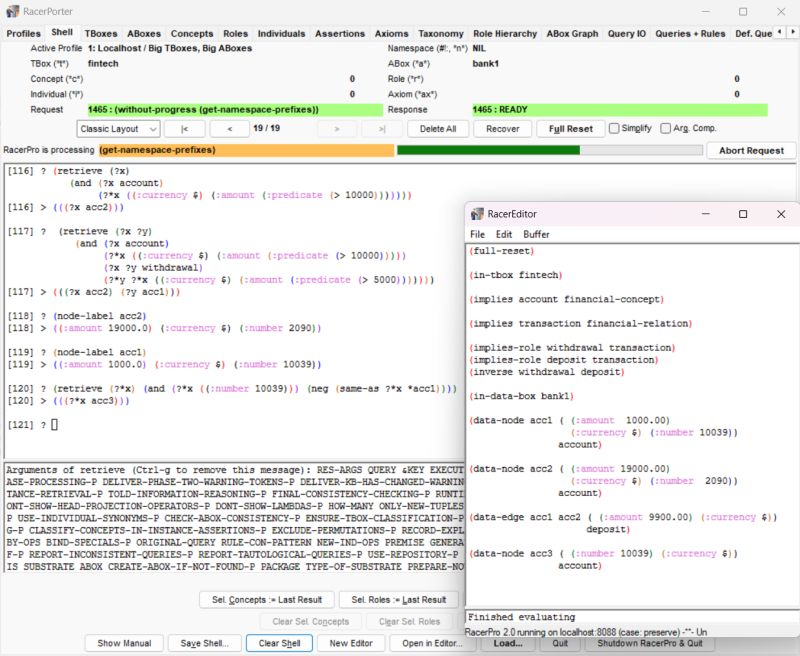
\includegraphics[width=0.9\linewidth]{pgraph-example.jpeg}
  \caption{A property graph built and queried in \racer{}~2.0 (RacerPorter). Nodes \texttt{acc1}--\texttt{acc3} and the \texttt{deposit} edge carry key--value property maps; \nrql{} filters on node \emph{and} edge properties and traverses the \texttt{deposit}/\texttt{withdrawal} (inverse) edge, while node types (\texttt{account}) are \owl{}/DL concepts and edge labels are DL roles.}\label{fig:pg}
\end{figure}

Two things are notable. First, this is a bona fide property graph---typed nodes and typed directed edges, both with key--value property maps, queried directly---and it predates the \emph{term} ``property graph.'' Second, and more distinctively, it is a property graph \emph{loosely coupled to a description-logic reasoner}: the node type \texttt{account} is a \tbox{} concept ($\texttt{account}\sqsubseteq\texttt{financial-concept}$) and the edge labels \texttt{deposit}/\texttt{withdrawal} are \tbox{} roles related by \texttt{inverse}, so a hybrid \nrql{} query mixes property-graph pattern matching with \owl{}/DL concept and role reasoning, inverses, and \naf{}. \textbf{We are aware of no prior or contemporary system that combined a queryable property graph with a tableau DL reasoner this way.} The substrate also answers the motivation directly: attaching \texttt{:amount}/\texttt{:currency} to the \texttt{deposit} \emph{relationship} is awkward in \rdf{} or DL (it forces reification or n-ary workarounds), which is exactly the shortcoming property graphs were meant to fix. This is not a paper exercise: the entire session of Figure~\ref{fig:pg} was reproduced live on \racer{}~2.0, returning the answers shown (transcript in the accompanying repository).

\subsection{Priority, calibrated as in \S\ref{sec:priority}}
The attributed/labeled-graph database \emph{model} is much older than 2005: Kuper and Vardi's Logical Data Model (1984) \cite{kupervardi}, the GOOD and hypernode models (1990) \cite{levene}, and especially G\"uting's \emph{GraphDB} (1994) \cite{guting}---which already modelled graphs with attributes on nodes and edges, with a query language, motivated by transportation networks---are recognizably graph-with-attributes models, surveyed by Angles and Gutierrez \cite{angles2008}. The branded model and the term came later: the Neo4j labeled-property-graph model was sketched around 2000 and released publicly around 2007, ``property graph'' was coined by Rodriguez and Neubauer in 2010 \cite{rodriguez2010}, and formal/standard treatments are later still (Angles' formal model, 2018; ISO GQL and SQL/PGQ, 2023--2024). \racer{}'s 2005 substrate therefore sits \emph{between} the academic graph-data-model tradition and the productized property-graph wave---an independent reinvention of a recurring idea.

So the calibrated claim is neither ``\racer{} invented property graphs'' (the model predates it by two decades) nor ``\racer{} influenced Cypher/GQL'' (no citation trail; these emerged from the graph-database and application world \cite{cypher2018}). It is the defensible middle: \racer{}'s data substrate is an early (2005), working, \emph{reasoning-coupled} property-graph store with edge-attribute querying---legitimate, and currently uncited, prior art for the combination of property graphs with description-logic reasoning, exhibiting the same convergent evolution that recurs throughout this history rather than any documented lineage.

\section{Answer to the main question}\label{sec:answer}

\begin{quote}
\textbf{\shacl{} did not introduce the ability to express closed-world integrity constraints over \owl{} data, required-property and qualified-cardinality constraints, annotation-governance constraints, or most datatype/string checks. Those were already expressible in \nrql{} via \naf{}, projection, rules, concrete-domain/datatype predicates, and the mirror/substrate layer \cite{adl04,nrql05,racerug}, and the underlying epistemic-query idea is older still \cite{epistemic,mknf}.}
\end{quote}

\noindent What \shacl{} did add, in decreasing order of how ``hard'' the novelty is:
\begin{enumerate}[leftmargin=2em]
  \item \textbf{Recursive shape conformance} as a first-class, possibly non-stratified fixpoint semantics, with NP-hard validation and undecidable satisfiability/containment in general \cite{recshacl,stableshacl,satcont}. This does not reduce to a single nonrecursive violation query.
  \item \textbf{Native unbounded regular paths}, provably outside the nonrecursive \naf{}-plus-projection fragment (Prop.~\ref{prop:paths}; \cite{ahoullman,libkin}).
  \item \textbf{An \rdf{}-term-native validation universe} (node kind, lexical form, language tags), conditional on what a \nrql{} substrate mirrors (\S\ref{sec:term}).
  \item \textbf{SPARQL algebra/term functions} when \shacl{}-SPARQL is used---conditional, since the common fragment still maps to hybrid \nrql{}.
  \item \textbf{A standardized conformance/validation-report model}---an organizational rather than expressivity gain.
\end{enumerate}

\noindent What was \emph{not} new: negated subqueries and universal closed-world queries, which \nrql{} realized via \texttt{NEG} over \texttt{PROJECT-TO} years before SPARQL~1.1 standardized them.

\section{Conclusion}\label{sec:conclusion}

A historically fair account should not say that \shacl{} was the first practical way to impose closed-world constraints on \owl{} data, nor that SPARQL~1.1 first made negated-subquery universal checks possible. \nrql{} supplied the essential mechanisms---\naf{}, projection, entailment-aware atoms, rules, concrete-domain predicates, aggregation, complex \tbox{} queries, and a hybrid substrate---and the mirror data substrate made \owl{} annotations and told values queryable, dissolving the false ``domain \abox{} versus ontology metadata'' boundary. \nrql{} deserves explicit recognition as prior art for negated projected subqueries in a practical \owl{} query engine, predating SPARQL~1.1 \cite{adl04,nrql05}.

The central difference is orientation. \nrql{} is a reasoner-integrated query-and-rule language that \emph{can be used to} validate, whose primary object is an answer set. \shacl{} is a validation language whose primary object is a conformance relation between data and shapes. That orientation buys \shacl{} two things that are not mere repackaging---recursive conformance semantics and native regular-path validation---plus \rdf{}-term primitives and a report model. It does not buy it the closed-world constraint idea, which the description-logic tradition and \nrql{} already had. What remains genuinely open, in both directions, is \emph{influence}: the conceptual debt is clear at the level of prior art and anticipation, but no citation trail establishes that SPARQL~1.1, \shacl{}, or Cypher built directly on \nrql{}.

\appendix
\section{Manual evidence, summarized}\label{sec:appendix}
The source points from the uploaded manuals most relevant to the comparison:
\begin{enumerate}[leftmargin=2em]
  \item \nrql{} described historically as an expressive DL query language with conjunctive queries, variables over named objects, \naf{}, projection, group-by, aggregation \cite[p.~4]{racerug}.
  \item Feature summary: atoms combine with \texttt{and}/\texttt{union}/\texttt{neg}/\texttt{project-to}; positive variables bind by entailment; \naf{} and classical negation; concrete-domain and datatype/annotation retrieval; projection and aggregation; hybrid substrate queries; the autoepistemic characterization \cite[pp.~81--84]{racerug}.
  \item \naf{} section: classical negation vs.\ \naf{}; missing-known-child idiom with \texttt{project-to} and \texttt{has-known-successor} \cite[pp.~113--120]{racerug}.
  \item Rules: query-body antecedents, generalized \abox{} consequents, individual creation, non-monotonicity \cite[pp.~125--127]{racerug}; \texttt{firerule} as the analogue of \texttt{retrieve} \cite[pp.~160--161]{racerrm}.
  \item Substrate: node/edge-labeled directed graph associated with an \abox{}; hybrid queries over both \cite[pp.~133--137]{racerug}.
  \item Mirror data substrate: substrate objects for \abox{} and \owl{} elements; \owl{} annotation/datatype markers; annotation/told values queryable as substrate nodes \cite[pp.~137--143]{racerug}.
  \item \texttt{NEG} over \texttt{project-to} and over defined queries: the negated-subquery idiom for closed-world universal constraints \cite[pp.~119--122]{racerug}.
\end{enumerate}

\begin{thebibliography}{99}

\bibitem{racerug}
Racer Systems GmbH \& Co.\ KG. \emph{RacerPro User's Guide Version 2.0}. October 24, 2012. \url{https://github.com/lambdamikel/Racer/tree/master/doc}. (Page numbers in this report are the printed page numbers of this edition; syntax was verified against \S4.1.9, pp.~150--153.)

\bibitem{racerrm}
Racer Systems GmbH \& Co.\ KG. \emph{RacerPro Reference Manual Version 1.9}. October 12, 2010. \url{https://github.com/lambdamikel/Racer/tree/master/doc}.

\bibitem{adl04}
Volker Haarslev, Ralf M\"oller, and Michael Wessel. Querying the Semantic Web with Racer~+~\nrql{}. In \emph{Proc.\ KI-2004 International Workshop on Applications of Description Logics (ADL'04)}, Ulm, Germany, September 2004.

\bibitem{nrql05}
Michael Wessel and Ralf M\"oller. A High Performance Semantic Web Query Answering Engine. In \emph{Proc.\ 2005 International Workshop on Description Logics (DL~2005)}, CEUR-WS Vol.~147, 2005.

\bibitem{epistemic}
Francesco M. Donini, Maurizio Lenzerini, Daniele Nardi, Werner Nutt, and Andrea Schaerf. An Epistemic Operator for Description Logics. \emph{Artificial Intelligence}, 100(1--2):225--274, 1998.

\bibitem{mknf}
Francesco M. Donini, Daniele Nardi, and Riccardo Rosati. Description Logics of Minimal Knowledge and Negation as Failure. \emph{ACM Transactions on Computational Logic}, 3(2):177--225, 2002.

\bibitem{eqllite}
Diego Calvanese, Giuseppe De Giacomo, Domenico Lembo, Maurizio Lenzerini, and Riccardo Rosati. EQL-Lite: Effective First-Order Query Processing in Description Logics. In \emph{Proc.\ 20th International Joint Conference on Artificial Intelligence (IJCAI 2007)}, pages 274--279, 2007.

\bibitem{rql}
Gregory Karvounarakis, Sofia Alexaki, Vassilis Christophides, Dimitris Plexousakis, and Michel Scholl. RQL: A Declarative Query Language for RDF. In \emph{Proc.\ 11th International World Wide Web Conference (WWW 2002)}, pages 592--603, 2002.

\bibitem{rdql}
Andy Seaborne. \emph{RDQL --- A Query Language for RDF}. W3C Member Submission, 9 January 2004. \url{https://www.w3.org/submissions/2004/SUBM-RDQL-20040109/}.

\bibitem{sparql10}
Eric Prud'hommeaux and Andy Seaborne, editors. \emph{SPARQL Query Language for RDF}. W3C Recommendation, 15 January 2008. \url{https://www.w3.org/TR/rdf-sparql-query/}.

\bibitem{sparql}
Steve Harris and Andy Seaborne, editors. \emph{SPARQL 1.1 Query Language}. W3C Recommendation, 21 March 2013. \url{https://www.w3.org/TR/sparql11-query/}.

\bibitem{shacl}
Holger Knublauch and Dimitris Kontokostas, editors. \emph{Shapes Constraint Language (SHACL)}. W3C Recommendation, 20 July 2017. \url{https://www.w3.org/TR/shacl/}.

\bibitem{shaclaf}
Holger Knublauch, Dimitris Kontokostas, et al. \emph{SHACL Advanced Features}. W3C Working Group Note, 8 June 2017. \url{https://www.w3.org/TR/shacl-af/}.

\bibitem{shex}
Eric Prud'hommeaux, Jose Emilio Labra Gayo, and Harold Solbrig. Shape Expressions: An RDF Validation and Transformation Language. In \emph{Proc.\ 10th International Conference on Semantic Systems (SEMANTICS 2014)}, pages 32--40, 2014.

\bibitem{spin}
Holger Knublauch. \emph{SPIN --- Modeling Vocabulary}. W3C Member Submission, 22 February 2011. \url{https://www.w3.org/Submission/spin-modeling/}.

\bibitem{recshacl}
Julien Corman, Juan L. Reutter, and Ognjen Savkovi\'c. Semantics and Validation of Recursive SHACL. In \emph{Proc.\ 17th International Semantic Web Conference (ISWC 2018)}, LNCS 11136, pages 318--336, 2018.

\bibitem{stableshacl}
Medina Andre\c{s}el, Julien Corman, Magdalena Ortiz, Juan L. Reutter, Ognjen Savkovi\'c, and Mantas \v{S}imkus. Stable Model Semantics for Recursive SHACL. In \emph{Proc.\ The Web Conference 2020 (WWW 2020)}, pages 1570--1580, 2020.

\bibitem{wfshacl}
Cem Okulmus et al. SHACL Validation under the Well-founded Semantics. In \emph{Proc.\ 21st International Conference on Principles of Knowledge Representation and Reasoning (KR 2024)}, 2024.

\bibitem{satcont}
Paolo Pareti, George Konstantinidis, Fabio Mogavero, and Timothy J. Norman. SHACL Satisfiability and Containment. In \emph{Proc.\ 19th International Semantic Web Conference (ISWC 2020)}, LNCS 12506, pages 474--493, 2020.

\bibitem{ahoullman}
Alfred V. Aho and Jeffrey D. Ullman. The Universality of Data Retrieval Languages. In \emph{Proc.\ 6th ACM Symposium on Principles of Programming Languages (POPL 1979)}, pages 110--120, 1979.

\bibitem{libkin}
Leonid Libkin. \emph{Elements of Finite Model Theory}. Springer, 2004.

\bibitem{angles2008}
Renzo Angles and Claudio Gutierrez. Survey of Graph Database Models. \emph{ACM Computing Surveys}, 40(1), Article~1, 2008.

\bibitem{kupervardi}
Gabriel M. Kuper and Moshe Y. Vardi. A New Approach to Database Logic (The Logical Data Model). In \emph{Proc.\ 3rd ACM SIGACT-SIGMOD Symposium on Principles of Database Systems (PODS 1984)}, 1984; journal version \emph{ACM Transactions on Database Systems} 18(3):379--413, 1993.

\bibitem{levene}
Mark Levene and Alexandra Poulovassilis. The Hypernode Model and its Associated Query Language. In \emph{Proc.\ 5th Jerusalem Conference on Information Technology (JCIT)}, pages 520--530, 1990. See also the GOOD model: Marc Gyssens, Jan Paredaens, and Dirk Van Gucht, A Graph-Oriented Object Database Model, In \emph{Proc.\ 9th ACM Symposium on Principles of Database Systems (PODS 1990)}, pages 417--424.

\bibitem{guting}
Ralf Hartmut G\"uting. GraphDB: Modeling and Querying Graphs in Databases. In \emph{Proc.\ 20th International Conference on Very Large Data Bases (VLDB 1994)}, pages 297--308, 1994.

\bibitem{rodriguez2010}
Marko A. Rodriguez and Peter Neubauer. Constructions from Dots and Lines. \emph{Bulletin of the American Society for Information Science and Technology}, 36(6):35--41, 2010.

\bibitem{cypher2018}
Nadime Francis, Alastair Green, Paolo Guagliardo, Leonid Libkin, Tobias Lindaaker, Victor Marsault, Stefan Plantikow, Mats Rydberg, Petra Selmer, and Andr\'es Taylor. Cypher: An Evolving Query Language for Property Graphs. In \emph{Proc.\ 2018 International Conference on Management of Data (SIGMOD 2018)}, pages 1433--1445, 2018.

\end{thebibliography}

\end{document}
